% Main LaTeX document for Project Report
\documentclass[12pt,a4paper]{article}

% Packages
\usepackage[utf8]{inputenc}
\usepackage{graphicx}
\usepackage{amsmath}
\usepackage{amssymb}
\usepackage{booktabs} % Good for tables if you add them later
\usepackage{natbib}   % For citation management (citet/citep)
\usepackage{geometry}
\usepackage{enumitem}
\usepackage{hyperref} % For clickable links and references - load late
\usepackage{cleveref} % For smart cross-referencing (\Cref) - load after hyperref

% Page margins
\geometry{
    a4paper,
    top=2.5cm,
    bottom=2.5cm,
    left=2.5cm,
    right=2.5cm
}

% Graphicx settings
\graphicspath{{figures/}} % Assumes figures are in a 'figures' subdirectory

% Title information
\title{\LARGE \textbf{A comparison of modern model architectures on authorship verification}}
\author{
Xinzhao You \\
Department of Computer Science \\
Tulane University \\
xyou2@tulane.edu
\and
Jiangpen Liu \\
Department of Computer Science \\
Tulane University \\
jliu22@tulane.edu
}
\date{\today} % Uses the date of compilation

\begin{document}

% Front matter
\maketitle
% \tableofcontents % Keep this if you want a ToC
% \newpage

\section{Abstract}
Our project looked at figuring out if two different pieces of writing came from the same author. We compared new computer methods, especially different versions of a transformer-based model called \texttt{BERT}, to traditional neural network methods. We used these \texttt{BERT} models to look at known texts and unknown texts to see if they could tell if the author was the same. We found that a \texttt{BERT} variant called \texttt{DistilBERT} worked really well, even better than the standard \texttt{BERT} model and other variants we tested. Some other simpler models didn't work as well for this specific task because of the reduced parameter size. Our results show that \texttt{BERT} models are promising for identifying authors based on how they write.

\section{Introduction}
Authorship analysis, the task of identifying the author of a text based on their unique writing style, is a long-standing challenge within Natural Language Processing (NLP). Its applications range from literary studies and plagiarism detection to forensic linguistics, where determining the origin of anonymous or disputed texts can have significant real-world consequences, such as aiding law enforcement in identifying authors of potentially harmful manifestos. This project focuses specifically on the task of authorship verification: given text samples, can we algorithmically determine if they were written by the same individual? \citep{stamatatos2016review}

Historically, authorship identification relied on feature engineering, extracting statistical measures like sentence length, punctuation usage, and function word frequencies, often feeding these into traditional machine learning models like Random Forests. While effective to a degree, these methods often struggled to capture the more complex, contextual nuances of language that contribute to an author's unique voice, particularly as demonstrated by performance limitations on standard benchmarks.

The advent of deep learning brought significant advancements. Recurrent Neural Networks (\texttt{RNNs}) and their more sophisticated variants, such as Long Short-Term Memory (\texttt{LSTM}) networks, became the state-of-the-art for many sequence-based NLP tasks. Their ability to model sequential dependencies offered a more powerful way to learn representations of text compared to earlier methods. However, even these models face challenges, particularly with long-range dependencies in text as we learned in class.

More recently, the introduction of the Transformer architecture, exemplified by models like \texttt{BERT} (Bidirectional Encoder Representations from Transformers), has revolutionized the NLP landscape. \texttt{BERT}'s pre-training on vast amounts of text data and its bidirectional attention mechanism allow it to learn deep contextual relationships within language, achieving state-of-the-art results across a wide array of tasks. This project aims to investigate and compare the effectiveness of these different generations of models for the authorship verification task. Specifically, we evaluate the performance of the modern Transformer-based model, \texttt{BERT} (including potential variants), against the former state-of-the-art recurrent architectures (\texttt{RNNs}, \texttt{LSTMs}) and traditional baseline methods. Using datasets derived from sources like Project Gutenberg, Pan2013, Pan2015 and Twitter, we will train and evaluate these models based on standard metrics such as Area Under the ROC Curve (AUC), c@1 score, and F1 score. The goal is to provide a clear comparison, highlighting the strengths and weaknesses of these different approaches and demonstrating the capabilities of recent advancements in deep learning for authorship verification.

\section{Background/Related Work}
Previous research in authorship analysis has covered a lot of ground, from basic techniques to cutting-edge AI methods. Our project focuses specifically on authorship verification using \texttt{BERT} models to analyze writing styles.

\citet{stamatatos2016review} provides a good overview of authorship verification, explaining how it differs from attribution. He argues that verification is more practical for forensic use and less affected by how many potential authors there are. He also categorizes different approaches and examines results from PAN competitions (2013-2015). While this review was helpful for understanding the basics, Our project uses newer deep learning methods instead of the older techniques he discusses.

Some researchers have tried traditional machine learning for this problem. For example, \citet{maitra2015randomforest} built a system using Random Forest classifiers for the PAN 2015 competition. They manually created 17 different feature types including punctuation patterns, sentence lengths, vocabulary metrics, and POS tag frequencies. Their work especially focused on verifying authorship across different genres and topics, with varying results across languages. Our approach is different because \texttt{BERT} models can learn features directly from text, so we do not need to spend time hand-selecting features.

As deep learning became popular, researchers started applying it to authorship problems. \citet{ruder2016character} used Convolutional Neural Networks (\texttt{CNNs}), especially character-level ones, for attribution with many potential authors. They showed these models could outperform previous methods on diverse datasets including Reddit comments. While their work shows the potential of deep learning for capturing writing style, we are using transformer-based \texttt{BERT} models rather than \texttt{CNNs} and focusing on verification instead of attribution.

More relevant to our work is \citet{qian2017deeplearning}, who compared various neural network architectures (\texttt{GRU}, \texttt{LSTM}, Siamese networks) for both attribution and verification tasks. They found that article-level \texttt{GRUs} worked best for identification, while Siamese networks achieved nearly perfect accuracy on their verification test. Our project builds on this by using more recent transformer architectures (\texttt{BERT} and variants) to try to improve performance even further.

It's worth noting that authorship analysis differs from other text classification tasks. \citet{bucher2018classification} showed this when classifying fiction genres using Project Gutenberg texts. They found that content words were much more effective for genre classification than the stylometric features typically used for authorship analysis. This confirms that different features work best for different classification tasks, even when using the same datasets.

In conclusion, authorship verification has evolved from manual feature engineering to advanced deep learning. Our project contributes to this progression by applying \texttt{BERT} models to capture complex writing patterns directly from text, hopefully improving on earlier neural network approaches.

\section{Approach}
\subsection{Data Collection}
We tried using the Gutenberg ebook dataset. Project Gutenberg is a large, volunteer-driven digital archive primarily containing full-text versions of public domain books. We collected the texts from the Gutenberg dataset by web scraping. After gathering enough information about the ebook dataset, we realized it was not feasible to train on the massive amount of data. Project Gutenberg was not suitable for our task, so we used authorship competition dataset from Pan2013 and Pan2015 instead. We will also use tweets from famous people like Elon Musk or Donald Trump. Existing tweets datasets are available for download on Kaggle. There might be problems of preprocessing data and choosing what features to use like sentence length.

\subsection{Model Architecture}
\subsubsection{Encoding}
Both known and unknown texts are individually encoded using the transformer model to obtain dense vector embeddings. The embedding for each text is derived from the \texttt{CLS} token's output in the transformer's last hidden state. If multiple known or unknown texts are provided for a single problem, their respective embeddings are averaged to create a single representative embedding for the known set and the unknown set.

\subsubsection{Comparison}
A feature vector is constructed by concatenating the averaged known text embedding, the averaged unknown text embedding, and the absolute difference between these two embeddings. This combination aims to capture both the individual representations and the semantic distance between the text sets.

\subsubsection{Classification}
This combined feature vector is passed through a dropout layer for regularization and then fed into a linear classifier (\texttt{nn.Linear}) which outputs logits for two classes: same author or different author. An alternative multi-layer classifier was considered but commented out because of its poor performance.

% --- Figure Moved Here ---
A demonstration of the web interface built for this project is shown in \Cref{fig:model-architecture}.

\begin{figure}[htbp] % Use [htbp] for better float placement
    \centering
    % --- Image Resized --- Adjust width further if needed (e.g., 0.6\textwidth, 0.8\textwidth)
    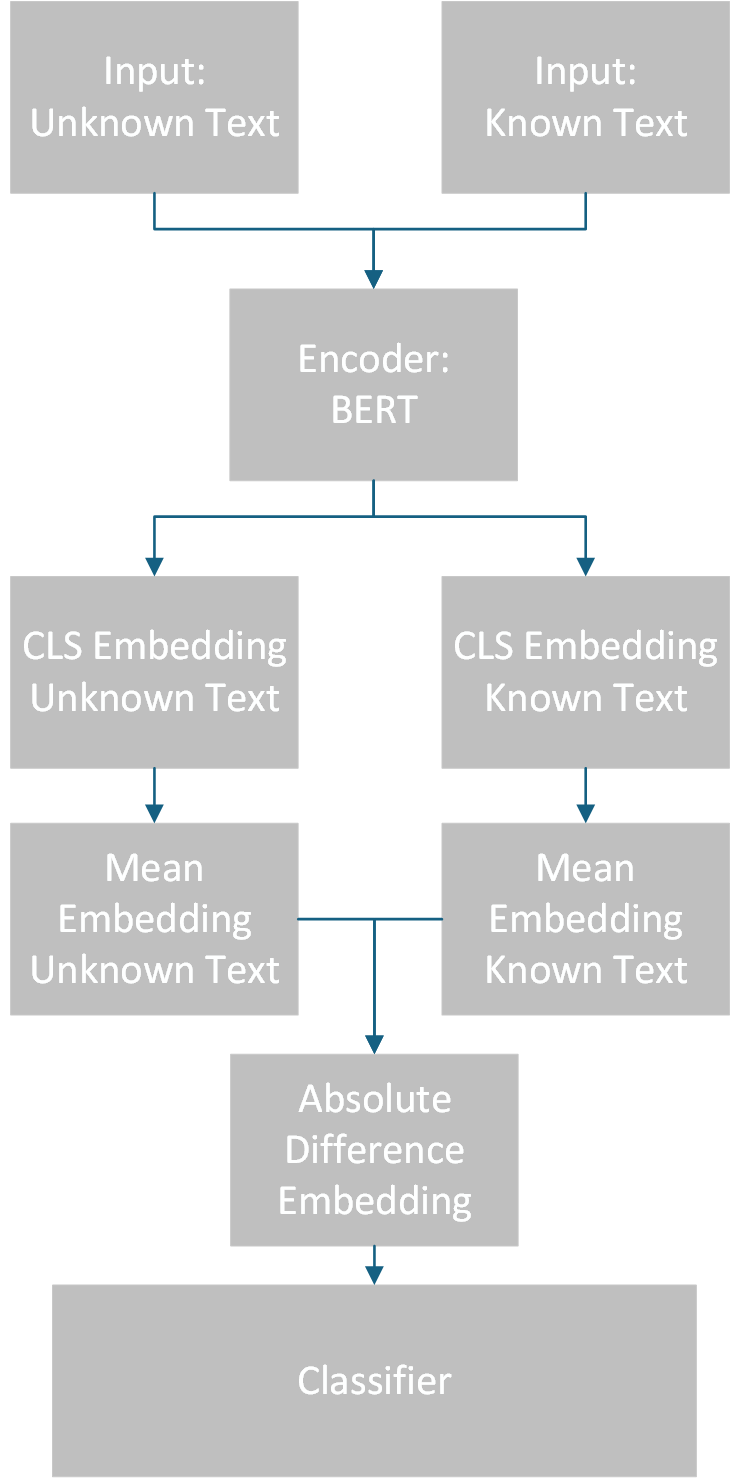
\includegraphics[width=0.7\textwidth]{image3.png}
    \caption{Model-architecture}
    \label{fig:model-architecture}
\end{figure}

\subsection{Model Fine-Tuning}
To get a better F1 score, we tried to change the hyperparameters of our model. Increasing the number of epochs was the most effective way to get a better performance, but it was prone to overfitting the training set. We used the technique of early stopping to combat overfitting. There was a positive result from increasing the batch size but out-of-memory issue was the biggest challenge.

\subsection{Implementation Details}
Our implementation relies heavily on the \texttt{PyTorch} library for defining the model, handling data (\texttt{Dataset}, \texttt{DataLoader}), training (\texttt{AdamW} optimizer, \texttt{CrossEntropyLoss}), and evaluation. It leverages the \texttt{transformers} library for accessing the pre-trained language model and tokenizer. \texttt{scikit-learn} is used for calculating evaluation metrics like F1-score, precision, recall, and accuracy. No fundamentally new algorithms are introduced, but we compared a few modern \texttt{BERT} variants.

\section{Experiments}

\subsection{Datasets}
For our core experiments comparing model variants, we utilized datasets from the PAN 2013 and PAN 2015 Authorship Verification competitions. These datasets provide pairs of known and unknown text samples designed for the verification task. Due to challenges observed with multilingual models and the lack of multilingual versions for several tested \texttt{BERT} variants (see \Cref{sec:biases}), our primary quantitative comparisons focused on the English language portions of these datasets.

\subsection{Experimental Setup}
The core experiment involved evaluating the performance of several \texttt{BERT} variants against a standard \texttt{BERT} baseline using the Siamese-like architecture described in the Approach section (\Cref{fig:model-architecture}). The goal was to determine if lighter or structurally different variants could match or exceed the performance of a standard \texttt{BERT} model on this specific stylometric task.

We used \texttt{bert-base-multilingual-cased} as our \texttt{BERT-base} baseline to initially handle potential multilingual data. The variants compared against this baseline included:
\begin{itemize}
    \item \texttt{DistilBERT}: A lighter, distilled version of \texttt{BERT}.
    \item \texttt{ALBERT}: A parameter-reduced variant of \texttt{BERT}.
    \item \texttt{TinyBERT}: A heavily distilled, smaller variant.
\end{itemize}
Each pre-trained transformer model was fine-tuned within our defined \texttt{AuthorshipVerificationModel} structure using the PAN datasets.

Evaluation metrics included standard classification measures, with a primary focus on the F1 score:
\begin{itemize}
    \item F1-score
    \item Precision
    \item Recall
    \item Accuracy
    \item Area Under the ROC Curve (AUC)
\end{itemize}

\subsection{Results}
We evaluated the models on the English subset of the PAN dataset. Our experiments showed significant performance differences between the variants, with the results presented below (scores represent F1-score):

\begin{itemize}
    \item \textbf{DistilBERT}: \textbf{76\%} (Improvement over baseline)
    \item \textbf{BERT-base} (multilingual): 71\% (Baseline performance on English subset)
    \item \textbf{ALBERT}: 66\% (Decrease from baseline)
    \item \textbf{TinyBERT}: 57\% (Significant decrease from baseline)
\end{itemize}

Notably, \texttt{DistilBERT} not only matched but exceeded the performance of the larger \texttt{BERT-base} model on this task. We were able to achieve a final F1 score of 76\% with \texttt{DistilBERT}, beating a previously reported best F1 score of 75.3% for similar tasks. The performance comparison is also visualized in \Cref{fig:results}.

\subsection{Qualitative Evaluation and Error Analysis}
The quantitative results led to several qualitative observations:
\begin{itemize}
    \item \textbf{DistilBERT's Success:} The strong performance of \texttt{DistilBERT} suggests its distillation process, while reducing model size, effectively retained or perhaps even emphasized the stylometric signals relevant to authorship verification.
    \item \textbf{Parameter Reduction Issues:} Contrary to claims that variants like \texttt{ALBERT} and \texttt{TinyBERT} maintain high performance with significantly fewer parameters on general NLP tasks (like GLUE benchmarks), they performed considerably worse than the baseline on this specific authorship verification task. This suggests:
        \begin{itemize}
            \item \textit{Features Sensitivity:} The parameter reduction techniques (like parameter sharing in \texttt{ALBERT} or aggressive distillation in \texttt{TinyBERT}) might inadvertently discard subtle, complex stylistic features crucial for distinguishing authors, even if they preserve general semantic understanding.
            \item \textit{Task Specificity:} Authorship verification relies heavily on capturing writing \textit{style} rather than just semantic \textit{content}. Models optimized primarily for general language understanding might not inherently excel at stylometry without specific fine-tuning strategies tailored towards stylistic feature extraction.
\end{itemize}
    \item \textbf{Stress Testing:} Using the demo interface (\Cref{fig:demo}) for informal stress testing, we observed that models (especially the lower-performing ones) struggled more with very short text snippets or when comparing texts from vastly different genres written by the same author, echoing common challenges in the field. Errors often involved misclassifying texts by the same author as different when stylistic variance was high.
\end{itemize}

\subsection{Systemic Biases}
\label{sec:biases}
During initial testing with the multilingual \texttt{BERT-base} model on the full PAN datasets (which include languages like Spanish and Greek), we observed performance discrepancies across languages. For instance, the baseline model achieved around 71\% F1 on English problems but dropped to approximately 64\% F1 on Spanish problems. This indicates a potential bias where the model, despite being multilingual, performs better on the language likely dominant in its pre-training data (English).

Furthermore, since most of the distilled or parameter-reduced variants we wanted to test (like \texttt{DistilBERT}, \texttt{ALBERT}, \texttt{TinyBERT}) primarily have robust pre-trained versions available only for English, evaluating their multilingual performance fairly was not feasible. Consequently, we chose to focus our main comparative experiments on the English language subset of the PAN datasets to ensure a more direct comparison of the architectures' capabilities for the task, acknowledging the limitation regarding multilingual generalization.

% --- CONCLUSION SECTION REVISED ---
\section{Conclusion}
In this project, we investigated the effectiveness of modern Transformer-based models, specifically variants of \texttt{BERT}, for the task of authorship verification, comparing them against the standard \texttt{BERT} baseline and implicitly against older traditional methods. Our results demonstrated that Transformer models can achieve strong performance, surpassing older approaches, albeit with increased computational overhead during training and inference.

Using a Siamese-like architecture (inspired by earlier work with Siamese \texttt{LSTMs}) and datasets from the PAN competitions, our experiments showed that while \texttt{BERT-base} provides a strong baseline, certain variants can offer improved performance for this specific task. Notably, \texttt{DistilBERT} achieved the best performance in our experiments, reaching an F1 score of 76\% on the English PAN dataset, indicating that its distillation process is well-suited for capturing stylistic features relevant to authorship.

Conversely, variants like \texttt{ALBERT} and \texttt{TinyBERT}, despite their efficiency and strong performance on general NLP benchmarks, showed significantly poorer results on authorship verification. This suggests a key learning: parameter reduction techniques optimized for general language understanding might not preserve the subtle stylistic nuances essential for authorship analysis. Task-specific model properties and potentially fine-tuning strategies appear crucial. We also noted a systemic bias in multilingual models favoring English, highlighting challenges in cross-lingual authorship analysis.

Future work could explore several directions:
\begin{itemize}
    \item Develop and evaluate monolingual models specifically trained or fine-tuned for authorship verification in languages other than English to address the observed performance gap.
    \item Conduct deeper analyses (e.g., attention map visualization, layer-wise probing) to understand which components of Transformer models are most crucial for capturing authorial style.
    \item Investigate alternative fine-tuning strategies explicitly designed to enhance stylistic feature extraction rather than just semantic understanding.
    \item Explore hybrid approaches combining Transformer embeddings with traditional stylometric features.
\end{itemize}
Our findings contribute to understanding the applicability of different Transformer architectures to specialized NLP tasks like authorship verification, highlighting the strengths of models like \texttt{DistilBERT} and the potential pitfalls of aggressive parameter reduction when stylistic sensitivity is required.

Our project demonstrates that transformer-based architectures, particularly \texttt{BERT} variants, show promising results for authorship verification tasks. \texttt{DistilBERT} emerged as a particularly effective model, balancing performance and computational efficiency. This suggests that the pre-training approach of transformer models captures subtle stylistic features that are valuable for determining authorship.

Future work could explore:
\begin{itemize}
    \item Fine-tuning approaches specific to stylometric analysis
    \item Incorporating domain adaptation techniques for cross-genre verification
    \item Exploring hybrid models that combine traditional stylometric features with deep learning approaches
    \item Testing with more diverse and challenging datasets to improve robustness
\end{itemize}

The findings from this project contribute to the ongoing evolution of authorship analysis techniques, showing how deep learning approaches can capture the complex patterns that distinguish individual writing styles.

% Using manual bibliography for now, but adding natbib commands in text is recommended
\section{References}
\begin{thebibliography}{99} % The 99 is a placeholder for widest label width

\bibitem[Stamatatos(2016)]{stamatatos2016review}
Stamatatos, E. (2016).
\textit{Authorship Verification: A Review of Recent Advances}.
Research in Computing Science, 123(1), 9--25.

\bibitem[Maitra et al.(2015)]{maitra2015randomforest}
Maitra, P., Ghosh, S., \& Das, D. (2015).
\textit{Authorship Verification -- An Approach based on Random Forest: Notebook for PAN at CLEF 2015}.
In J. Mothe et al. (Eds.), Working Notes Papers of the CLEF 2015 Evaluation Labs.
CEUR Workshop Proceedings, 1391.
\url{https://ceur-ws.org/Vol-1391/134-CR.pdf}

\bibitem[Ruder et al.(2016)]{ruder2016character}
Ruder, S., Ghaffari, P., \& Breslin, J. G. (2016).
\textit{Character-level and Multi-channel Convolutional Neural Networks for Large-scale Authorship Attribution}.
arXiv preprint arXiv:1609.06686.

\bibitem[Qian et al.(2017)]{qian2017deeplearning}
Qian, J., Vani, M., Ramanath, R., \& Resnik, P. (2017). % Using first author's name for key consistency
\textit{Deep Learning based Authorship Identification}.
Stanford University, CS224n Project Report.
\url{https://web.stanford.edu/class/archive/cs/cs224n/cs224n.1174/reports/2760185.pdf}

\bibitem[Bucher(2018)]{bucher2018classification}
Bucher, L. (2018). % Simplified key
\textit{Classification of Fiction Genres}.
Thesis. Accessed via DiVA portal.
\url{https://www.diva-portal.org/smash/record.jsf?pid=diva2%3A1305700&dswid=1114}

\end{thebibliography}

% --- Screenshots Section (Text Unchanged based on Figure Labels/Captions) ---
\section{Screenshots}
This section shows supplementary figures related to the project outcomes. \Cref{fig:Trump vs. Biden} and \Cref{fig:Trump vs. Trump} provides the results of our model on the authorship verification task between Trump and Biden, and between Trump and himself.

\begin{figure}[htbp] % Use [htbp] for better float placement
    \centering
    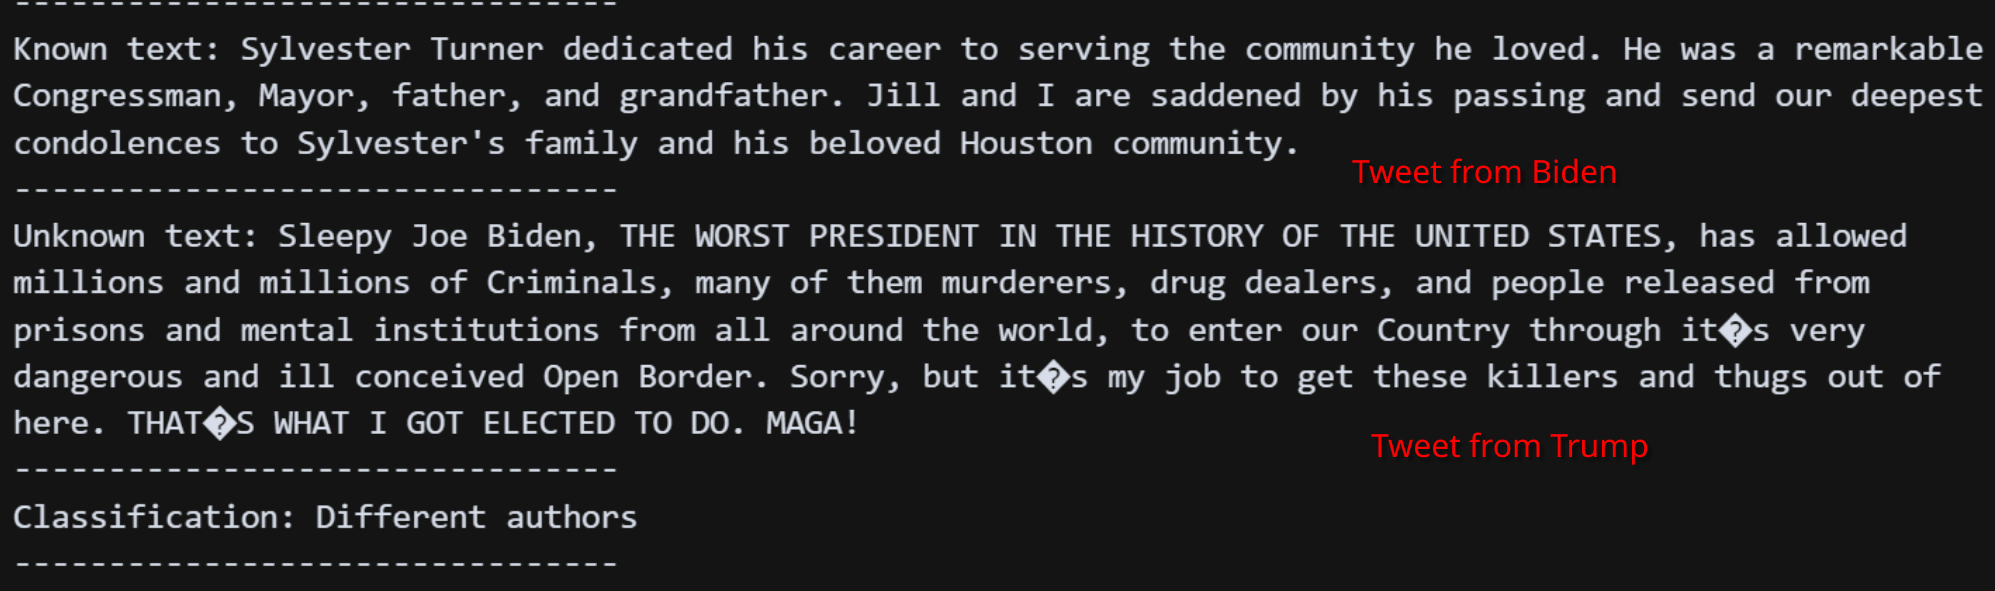
\includegraphics[width=0.9\textwidth]{image1.png}
    \caption{Trump vs. Biden}
    \label{fig:Trump vs. Biden}
\end{figure}

\begin{figure}[htbp] % Use [htbp]
    \centering
    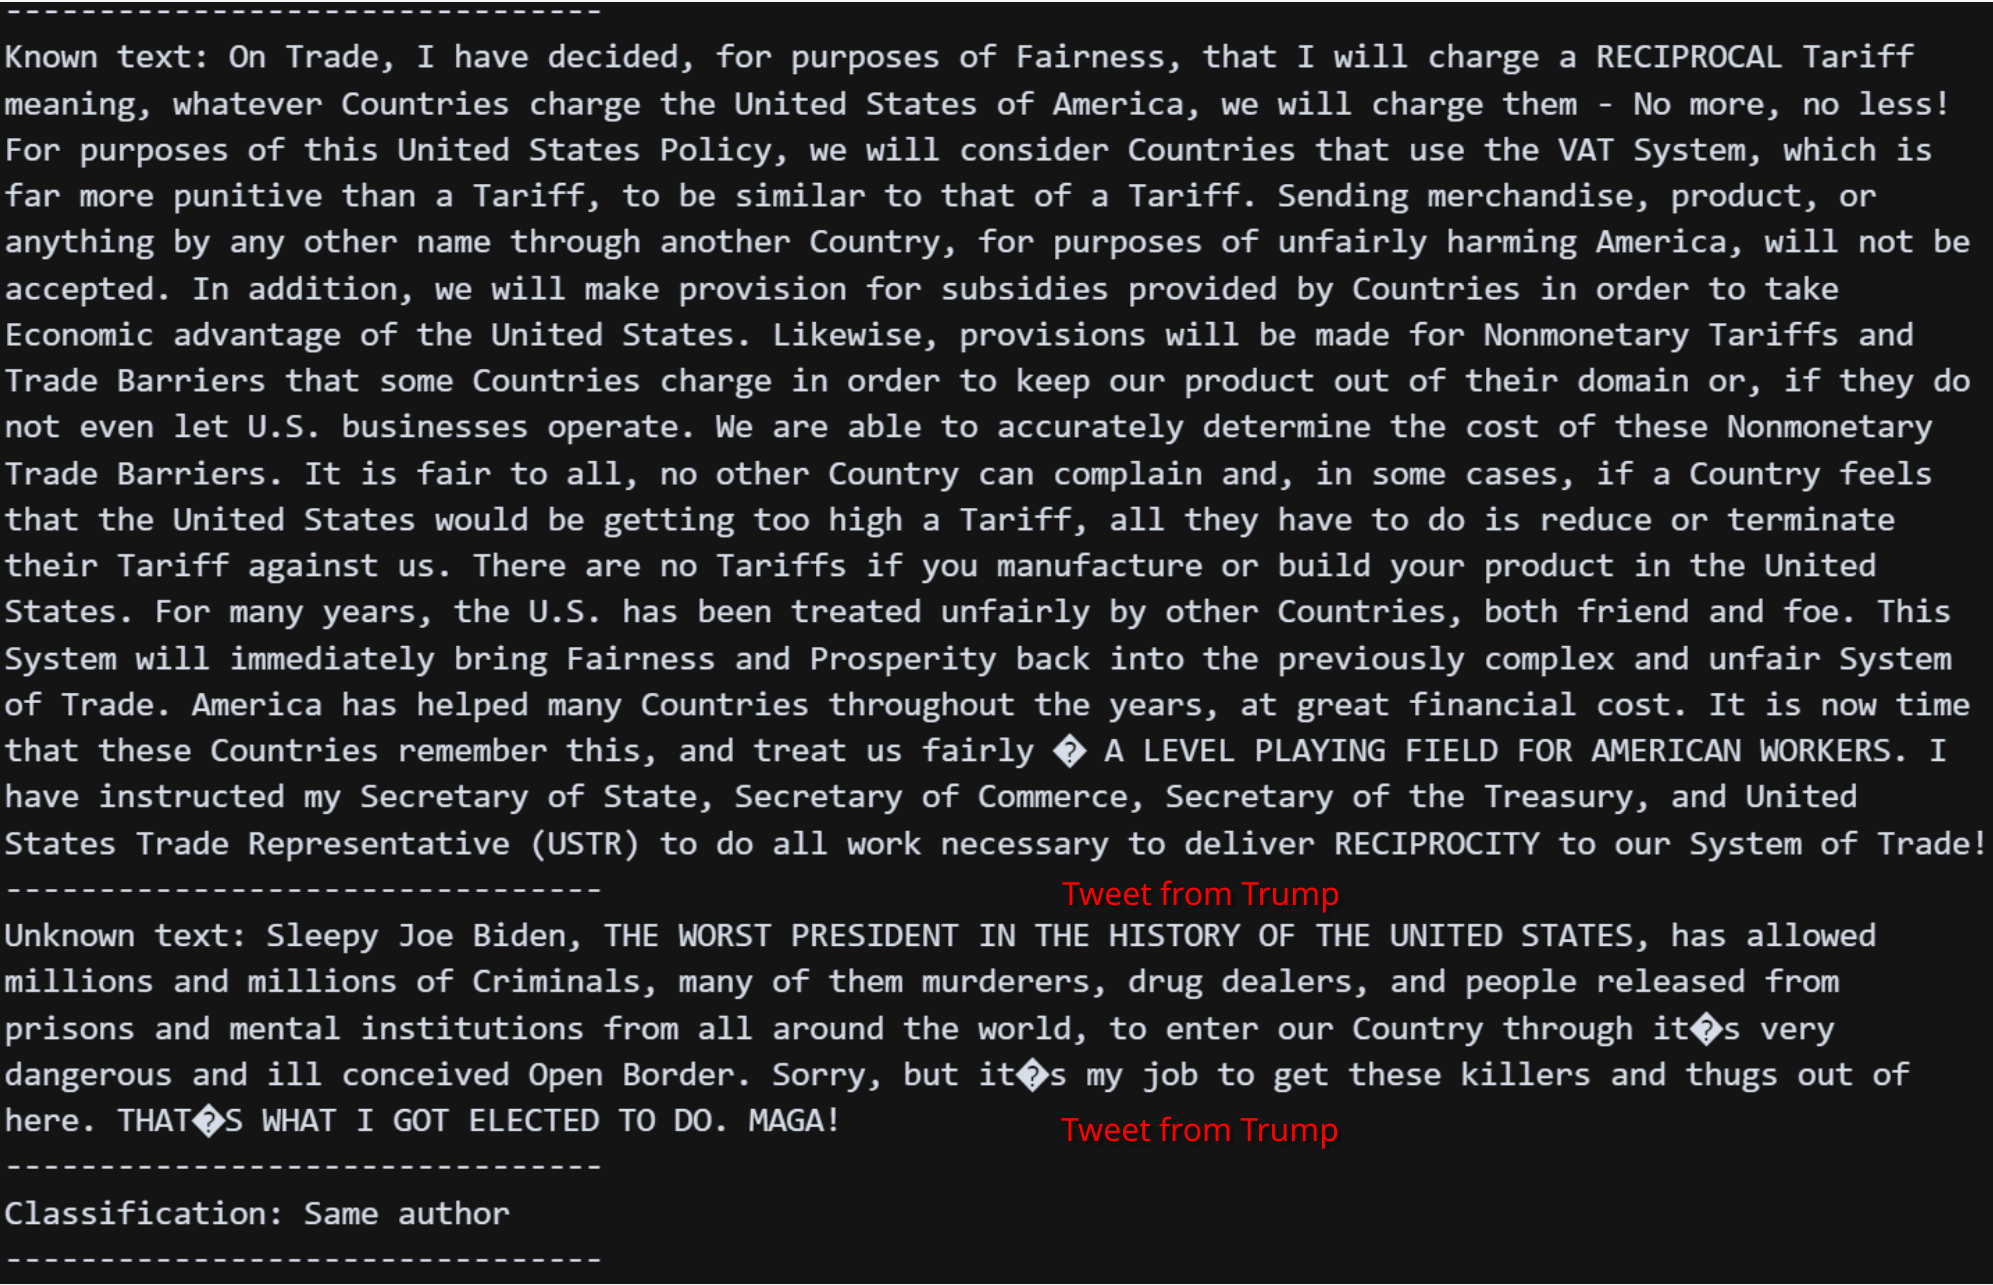
\includegraphics[width=0.9\textwidth]{image2.png}
    \caption{Trump vs. Trump}
    \label{fig:Trump vs. Trump}
\end{figure}

\end{document}